\chapter{Planteamiento del Problema}
En este capítulo se entrara en detalle sobre los términos relacionados al proyecto y se analizan 
trabajos anteriores sobre software enfocados en la enseñanza de programación de computadoras desde los 
60s hasta la actualidad. De igual manera, se define que atacaremos con este proyecto, una problemática y qué objetivos tiene el proyecto.

\section{Antecedentes}

\subsubsection{Videojuegos como método de enseñanza}
El área de \textit{serious games} puede pensarse como dos grandes áreas: entre ellas existe el \textit{edutainment}, aplicaciones informáticas con animaciones, elementos multimedia que muestran la información de una manera divertida; y los videojuegos, creados con la pretensión explícita de enseñar, incluyen el entrenamiento a base de simuladores, 
la transmisión de la información o incluso, la promoción de alguna idea o marca \cite{unknown2017a}. 
La principal diferencia para este es la difusión del contenido, el \textit{edutainment} prioriza 
la difusión de manera lúdica, mientras que los videojuegos serios deciden 
sacrificar la parte lúdica para explorar de mejor manera los conocimientos y lo hace de maneras más complejas \cite{unknown2017a}.
Mucho del desarrollo en el área de los \textit{serious games} fue en la milicia, aparte de ser de los primeros en adoptarlos. Estos se usan para el adiestramiento militar, sin contar con el número de simulaciones de distintos vehículos militares \cite{unknown2017a}. 
Asimismo, han existido \textit{serious games} de política, con diferentes propósitos, como la comunicación de ideas, criticar a oponentes o reproducir sus discursos. 
Otros ejemplos son los \textit{news games} que mezclan lo periodístico con la denuncia política y exponen una problemática de un determinado lugar y tiempo. 
Adicionalmente existen géneros como los \textit{advergames}, usados para publicidad, 
los de salud que permiten a los estudiantes aprender sin temor a equivocarse con un ser humano, los videojuegos artísticos y los videojuegos religiosos \cite{unknown2017a}.

\subsubsection{Evolución de la enseñanza de la programación}
Podemos notar como punto importante la creación de Pascal a finales de los 60s y principios de los 70s por parte de Niklaus Wirth, un lenguaje enfocado en la enseñanza de técnicas de programación, con una nueva metodología de programación denominada programación estructurada [2]. Sin embargo, no todo es tan claro, no ha existido un consenso de los métodos a utilizar y no ha existido alguno que se haya impuesto. 
Existen métodos para la enseñanza de otros paradigmas de programación como el funcional, el imperativo o el imperativo orientado a objetos; y dentro de estas divisiones hay quienes enseñan a programar mediante un lenguaje particular o quienes emplean un lenguaje algorítmico que pudiera adaptarse a otros lenguajes de programación [2].
Sin embargo, podemos destacar la existencia de algunas nuevas herramientas:

\subsubsection{LOGO}
\textit{LOGO} es un lenguaje de programación diseñado como una herramienta para aprender programación. 
Permite mover una \textit{tortuga} (originalmente una criatura robótica) a cualquier dirección 
mediante introducir comandos a la computadora \cite{logo_history} cómo se nota en la Figura~\ref{fig:logo_scrn}.

\begin{figure}[ht]
    \centering
    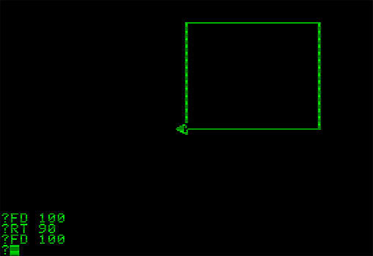
\includegraphics[width=0.5\textwidth]{logo}
     \caption{LOGO.}
    \label{fig:logo_scrn}
\end{figure}

\subsubsection{Pascal}
Lenguaje creado en 1970 por Niklaus Wirth para enseñar programación estructurada, 
paradigma de programación donde se pone énfasis en las 
estructuras condicionales y cíclicas, sin GOTO \cite{pascal_history}. 
Fue comúnmente usado durante la segunda mitad de los 70 y los 80 
debido a su disponibilidad en un gran número de computadoras, 
así como por su claridad y seguridad, no era raro que fuera usado para la 
producción de software.

\subsubsection{Python}
Diseñado por Guido Van Rossum originalmente estaba pensado 
para como un lenguaje de \textit{scripting} para el sistema operativo \textit{Amoeba} \cite{python_history}. 
Su ventaja en el ámbito educativo es su facilidad de uso, comúnmente descrito 
como poder programar en inglés y la gran cantidad de librerías que permiten 
crear cosas complejas de manera rápida.

\subsubsection{Lego WeDo 2.0}
Es un kit diseñado para introducir a niños y niñas a la robótica, 
construyen pequeños robots con \textit{LEGO} y de diferentes 
formas pueden programarlos para que se muevan. 
Normalmente hacen uso de programación por bloques.

\subsection{Trabajos relacionados}
En la actualidad, muchos programas para enseñar programación utilizan 
\textit{drag-and-drop} para realizar la tarea de programación, 
a esta se le conoce como \textit{block-based programming} \cite{block_based_programming}. 
Ejemplos de herramientas de esta categoría incluyen el entorno \textit{Scratch}, 
que permite crear pequeños juegos o animaciones con sus herramientas, 
como se nota en la figura~\ref{fig:scratch_scrn} y \textit{Code.org}, donde hay diversas actividades 
para aprender a programar.

\begin{figure}[ht]
    \centering
    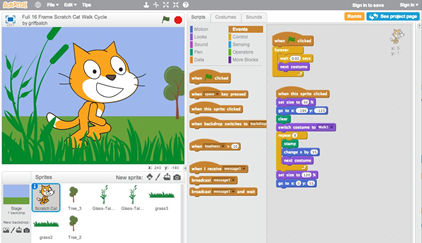
\includegraphics[width=0.5\textwidth]{scratch}
    \caption{El entorno de programación Scratch.}
    \label{fig:scratch_scrn}
\end{figure}

Similar, aunque a diferencia de este proyecto, \textit{Lego WeDo} va orientado a la robótica. Según la clase, eligen de una de las diferentes opciones disponibles para construir y los alumnos siguen unas instrucciones similares a otros \textit{kits} de \textit{LEGO}, y puede ser programado en \textit{Scratch} o en un software propio de \textit{LEGO} \cite{lego_wedo_explanation}. Incluye un \textit{hub} con conectividad \textit{bluetooth}, donde se pueden conectar sensores y motores \cite{lego_wedo_site}, como se puede ver en la figura~\ref{fig:wedo_kit}. El software de \textit{LEGO} es igual, \textit{block-based programming} e incluye sesiones donde los estudiantes aprenden de diversos temas y realizan actividades de programación relacionadas a estos. A diferencia de estos dos, en lugar de ser el profesor la principal fuerza para poner nuevos retos y enseñar nuevos conceptos, acudiremos a mecánicas vistas en videojuegos.

\begin{figure}[ht]
    \centering
    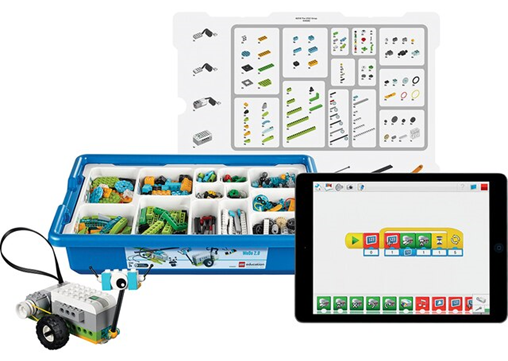
\includegraphics[width=0.5\textwidth]{wedo}
    \caption{Un kit de Lego WeDo.}
    \label{fig:wedo_kit}
\end{figure}

Por otro lado esta \textit{Kahoot!}, que es una plataforma de \textit{game-based learning} \cite{wang2015a}, esta permite a profesores poner \textit{quizzes}, de los cuales los estudiantes eligen la respuesta en sus teléfonos y en una pantalla más grande a la que tiene acceso el profesor se muestra la pregunta actual con sus posibles respuestas, así como la posición en la que están los alumnos entre cada pregunta, como se nota en la figura~\ref{fig:kahoot}. Este proyecto es útil para las evaluaciones, sin embargo, de manera similar a este el profesor tiene el control del tema a trabajar y lo controla desde un \textit{lobby}. 

\begin{figure}[ht]
    \centering
    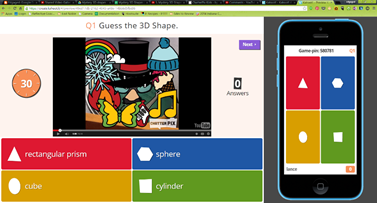
\includegraphics[width=0.5\textwidth]{images/kahoot.png}
    \caption{Kahoot!}
    \label{fig:kahoot}
\end{figure}

Hay una variedad de juegos de programación, como \textit{CodingGames}, que es un sitio de mini-juegos donde se ofrecen instrucciones sobre el punto del juego y cuenta con un \textit{IDE} para programar una solución para pasarlo. Asimismo, \textit{CodeCombat}, un juego de \textit{dungeon crawling} donde se debe programar para avanzar en el juego [10], hay aspecto \textit{multijugador} y al igual a \textit{Kahoot!} uno puede ser parte de un \textit{lobby} de una clase y el profesor puede ver el avance de sus alumnos, pero cada jugador avanza a su ritmo. Similarmente, en \textit{Screeps} un \textit{MMO} de estrategia para programadores de \textit{Javascript} y \textit{CheckIO}, se deben resolver problemas en \textit{Python} \cite{programming_games}. Sin embargo, todos están enfocados además en la enseñanza de un lenguaje de programación (\textit{Python} o \textit{Javascript} son opciones comunes), por lo que para un principiante puede ser un punto de contención adicional el aprender la sintaxis durante la práctica. Similarmente, en el área de \textit{edutainment} existen juegos como \textit{Human Resource Machine}, \textit{Hack ‘n’ Slash}, \textit{TIS-100}, donde a excepción del ultimo están enfocados a desarrollar una lógica para programar, \textit{TIS-100} agrega un lenguaje ensamblador con programación a base de \textit{nodos}, cada nodo solo acepta programas pequeños, se comunican varios nodos para crear programas más complejos, \textit{TIS-100} es más apto para enseñar sistemas distribuidos en lugar de programación básica.

\subsection{Lógica de programación}
La lógica de programación se refiere al desarrollo de secuencias a fin que al ejecutarse linealmente hasta su completitud realicen un objetivo o sea un algoritmo \cite{logica_programacion}, por ejemplo, una receta de cocina. Esta habilidad requiere el desarrollo de raciocinio lógico y estructurado, así como la capacidad de analizar la causa y efecto de cada paso del algoritmo, así como la capacidad de detectar errores y proponer mejoras.

\section{Definición del problema}
La enseñanza de programación es regularmente una dualidad con la enseñanza de un lenguaje de programación, donde se enfoca en la enseñanza de la sintaxis y en la enseñanza y práctica de hilar la lógica necesaria para crear un programa para computadoras, donde entran técnicas como [12]:
\begin{itemize}
    \item Descomposición de problemas complejos
    \item Reconocimiento de patrones para buscar similitudes entre problemas
    \item Abstracciones
    \item Algoritmos
\end{itemize}

La enseñanza de programación es un proceso complejo, donde el alumno tiene que acostumbrarse a razonar la forma de solucionar un problema (a base de descomposición) y aprender un lenguaje de programación con todas las idiosincrasias que este tenga, desarrollando los debidos modelos mentales sobre el funcionamiento del lenguaje y sobre la notación para resolver un problema \cite{mow-a}. La sintaxis de un lenguaje de programación puede ser complicado para un principiante, se ha encontrado que estos tienen dificultad para encontrar errores gramaticales en su código. Para esto, sería mejor dotar a alguien aprendiendo a programar con la habilidad de razonar problemas en un entorno donde no tengan que razonar mucho la sintaxis del lenguaje, y haya aspectos visuales que permitan al usuario experimentar programando y desarrollar los modelos mentales, pero reduzcan la carga cognitiva de usar una herramienta como un lenguaje de programación escrito por texto. 

\section{Objetivo general}
Desarrollar un videojuego multijugador que permita a estudiantes reforzar sus conocimientos de programación estructurada y mejorar sus habilidades de lógica de programación. 

\subsection{Objetivos específicos}

\begin{enumerate}
    \item Creación de un documento de diseño que defina el alcance del juego, sus componentes y subsistemas. Que permita a sus jugadores aprender programación estructurada.
    \item Crear un juego basado en este documento de diseño.
    \item Validar que el juego sea óptimo mostrando el juego a docentes de la materia y obteniendo retroalimentación.
\end{enumerate}

\section{Pregunta de Investigación}
¿El videojuego propuesto es óptimo para ser usado por maestros en el salón de clase?

\section{Justificación}
Un videojuego colaborativo permitiría tener ventajas como el desarrollo de las habilidades cognitivas, sociales en un ambiente de colaboración que permite a sus integrantes encontrar nuevas formas de atacar problemas, algunas de estas de especial importancia para la programación. 
Adicionalmente, los videojuegos son peculiarmente efectivos para la resolución de problemas, debido a que permiten “aprender haciendo” donde el proceso de aprendizaje es una constante práctica e interacción con tareas más complejas donde los jugadores encuentran reglas subyacentes que son de utilidad para resolver los problemas que nos plantee el juego \cite{monjelat-a}. Peculiarmente, este método de aprendizaje iterativo es muy cercana a la manera en la que resolvemos problemas en la vida diaria. Durante nuestro día a día regularmente resolvemos problemas por analogía, donde recurrimos a esquemas (paquetes de información sobre las propiedades del problema como: el conocimiento antes de intentar resolver el problema, a qué se quiere llegar, los posibles pasos y aquello que es permitido y las consecuencias de escoger incorrectamente) y se recupera el marco que se creó anteriormente para resolver este nuevo problema.
Un videojuego para la enseñanza de programación con los puntos anteriores, puede ser una excelente herramienta para la enseñanza en salones de clase de los elementos básicos de la programación y permitir a principiantes desarrollar la habilidad de resolver problemas. Adicionalmente, un videojuego corto puede ser una excelente herramienta para una clase de \textit{Hour of Code} (una propuesta para en una hora, introducir a pequeños o a grandes a la computación o a la programación).


\section{Delimitaciones y limitaciones}
\subsection{Delimitaciones}
\begin{itemize}
    \item Este videojuego se podrá jugar desde un navegador web, de preferencia en computadoras de escritorio o \textit{laptops}. Ante ello será programado en el \textit{engine} \textit{Unity3D} exportando al entorno \textit{WebGL}.
    \item El producto tendrá un tiempo de juego de 20 a 30 minutos de juego.
    \item Los \textit{puzzle} están enfocados a enseñar mediante educación JIT diferentes conceptos de programación procedimental y entrenar la lógica de programación.
    \item Se usó \textit{Mirror} como librería para manejar el multijugador.
\end{itemize}
\subsection{Limitaciones}
\begin{itemize}
    \item Se tuvo un límite de tiempo de desarrollo a 4 meses para acomodar la validación y
procesos adicionales.

\end{itemize}
